\section{Impegno orario}

Il tredicesimo gruppo composto da 7 studenti si impegna in toto a contribuire per ore \textbf{95} pro capite allo svolgimento del progetto didattico.

Suddette ore verranno suddivise come segue, tenendo conto dei ruoli definiti.

\begin{center}
    \begin{tabularx}{10cm}{X |l|l}
        \textbf{Ruolo}  & \textbf{Costo orario} & \textbf{Ore per ruolo} \\
        \hline
        Responsabile    & €30                   & 60                     \\
        Amministratore  & €20                   & 67                     \\
        Analista        & €25                   & 133                    \\
        Progettista     & €25                   & 153                    \\
        Programmatore   & €15                   & 152                    \\
        Verificatore    & €15                   & 100                    \\
        \hline
        \textbf{Totale} & €14064,75             & 665
    \end{tabularx}
\end{center}

Immaginiamo poi di spendere un \textbf{20\%} aggiuntivo di ore reali rispetto alle ore produttive qui sopra redatte. Questo rendimento tenderà a migliorare durante tutto lo svolgimento del progetto.

Le distribuzioni di costi e ore per ruolo è come segue.

\begin{minipage}[c][][c]{0.49\linewidth}
    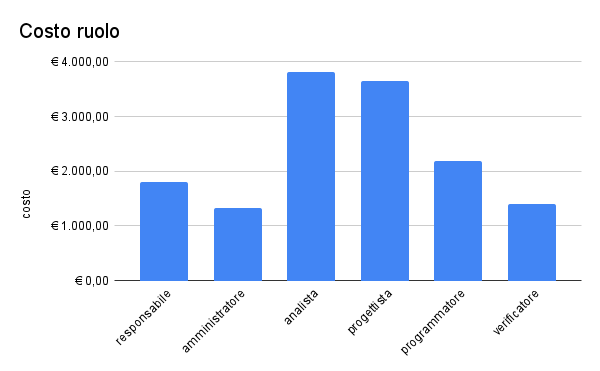
\includegraphics[width=\textwidth]{immagini/Costo ruolo.png}
\end{minipage}
\begin{minipage}[c][][c]{0.49\linewidth}
    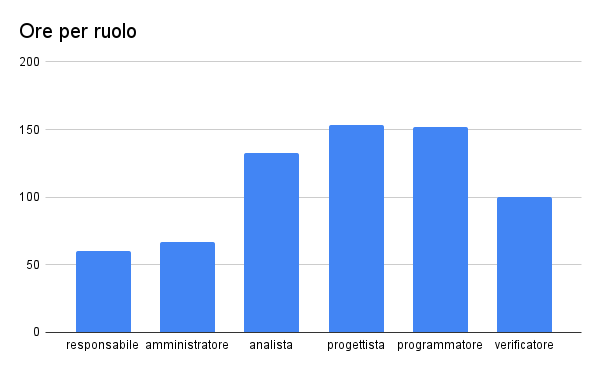
\includegraphics[width=\textwidth]{immagini/Ore per ruolo.png}
\end{minipage}

Ogni ruolo avrà inoltre rotazione costante e sistematica ma le ore preventivate per ogni studente si attestano a questi valori:

\begin{center}
    \begin{tabularx}{13cm}{X |l l l l l l| X}
        \textbf{Nome} & \textbf{re}\footnote{Responsabile}
        & \textbf{am}\footnote{Amministratore e amministratore di sistema}
        & \textbf{an}\footnote{Analista}
        & \textbf{pro}\footnote{Progettista}
        & \textbf{prog}\footnote{Programmatore}
        & \textbf{ve}\footnote{Verificatore}
        & \textbf{Totale} \\
        \hline
        Alessandro      & 9           & 8           & 18          & 24           & 20            & 16          & 95              \\
        Davide          & 9           & 10          & 18          & 22           & 23            & 13          & 95              \\
        Giorgio         & 8           & 9           & 20          & 22           & 23            & 13          & 95              \\
        Luca            & 9           & 10          & 18          & 22           & 20            & 16          & 95              \\
        Mattia          & 8           & 10          & 20          & 21           & 22            & 14          & 95              \\
        Michele         & 9           & 10          & 19          & 21           & 22            & 14          & 95              \\
        Samuel          & 8           & 10          & 20          & 21           & 22            & 14          & 95              \\
        \hline
        \textbf{Totale} & 60          & 67          & 133         & 153          & 152           & 100         & 665
    \end{tabularx}
\end{center}

\section{Ruoli e considerazioni}

\paragraph{Responsabile} Dopo attenta analisi il numero di ore di responsabile risulta ridotta in quanto ce ne sarà molto bisogno nelle fasi iniziali ma nel tempo la tendenza sarà quella dell'autogestione. Chiaramente il responsabile durante tutto il progetto sarà presente e farà da punto di contatto con il cliente ed il committente.

\paragraph{Amministratore} Sarà una delle figure più importanti nelle fasi di avviamento del progetto in quanto sarà suo onere improntare e controllare che tutte le procedure siano eseguite a regola d'arte e seguendo i corretti standard. Anche questa figura tenderà a sfumare con l'avvenire del progetto.

\paragraph{Analista}L'analista avendo l'onere di spianare la strada al progettista e al programmatore avrà bisogno di molto tempo così da poter rendere più agevole il compito ad essi. Avrà inoltre bisogno di molto tempo per documentare correttamente quali sono i bisogni del cliente.

\paragraph{Progettista} Abbiamo deciso di dedicare al progettista molte ore, poiché un'architettura ben strutturata rende il lavoro del programmatore più semplice e veloce da svolgere.

\paragraph{Programmatore} Sicuramente servià un buon tempo per stendere il codice in modo corretto.

\paragraph{Verificatore} Il verificatore dovrà assicurare molteplici attività di controllo e verifica durante tutto lo svolgimento. Non avrà quindi mai pace fino al compimento del progetto.

\section{Costi}

Il preventivo per la realizzazione del progetto ammonta quindi a €14064,75 che arrotondiamo per eccesso e tenendo a mente possibili imprevisti a \textbf{€14100,00}

\section{Consegna}

La previsione di consegna viene calcolando una media di \textbf{8} ore settimanali dedicate al progetto. Risultano quindi 12 settimane per terminare lo stesso.

Tenendo quindi conto anche di possibili imprevisti, giorni non lavorativi e cause di forza maggiore non ad ora preventivabili, la previsione di consegna chiavi in mano si attesta oggi al \textbf{26 aprile 2023}
